Poner que: comparamos con el benchmark de otros programas, comparar ese benchmark con dani, y que seguimos agrandando los tests de regresión para ir modificando con más confianza el código.

\section{Creimiento de los tests de regresión}


\section{Comparación con otros programas}


\section{Comparación con versión previa de DCS}
El principal foco del trabajo fue de brindar una mayor seguridad sobre la correctitud y completitud del approach novedoso de la exploración on the fly. Esto debía hacerse sin perder la buena performance que aportaba la técnica, con el foco de poder aplicarla a casos de mayor tamaño.

Para comparar la performance perdida por nuestros cambios al algoritmo, repetimos el benchmark diseñado por Daniel y lo comparamos con sus resultados. Aclaramos que el benchmark se corrió en un equipo de las mismas características que el usado en su momento por Daniel.

\begin{figure}[htb]
	\makebox[\linewidth][c]{%
		\begin{subfigure}[t]{.7\textwidth}
			\centering
			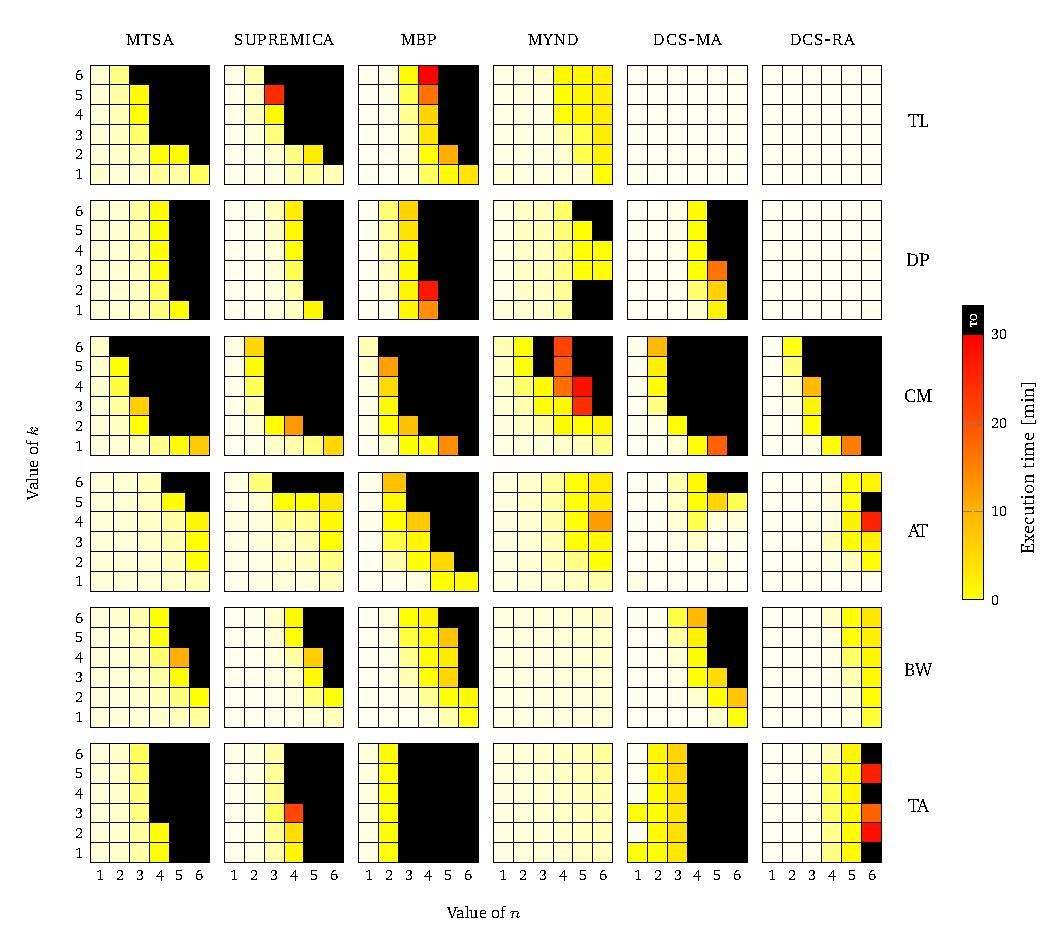
\includegraphics[width=\linewidth]{figures/nuestrosResults/detailed.pdf}  
			\caption{nueva performance}
			\label{fig:nuevoDetailed}
		\end{subfigure}
		\begin{subfigure}[t]{.7\textwidth}
			\centering
			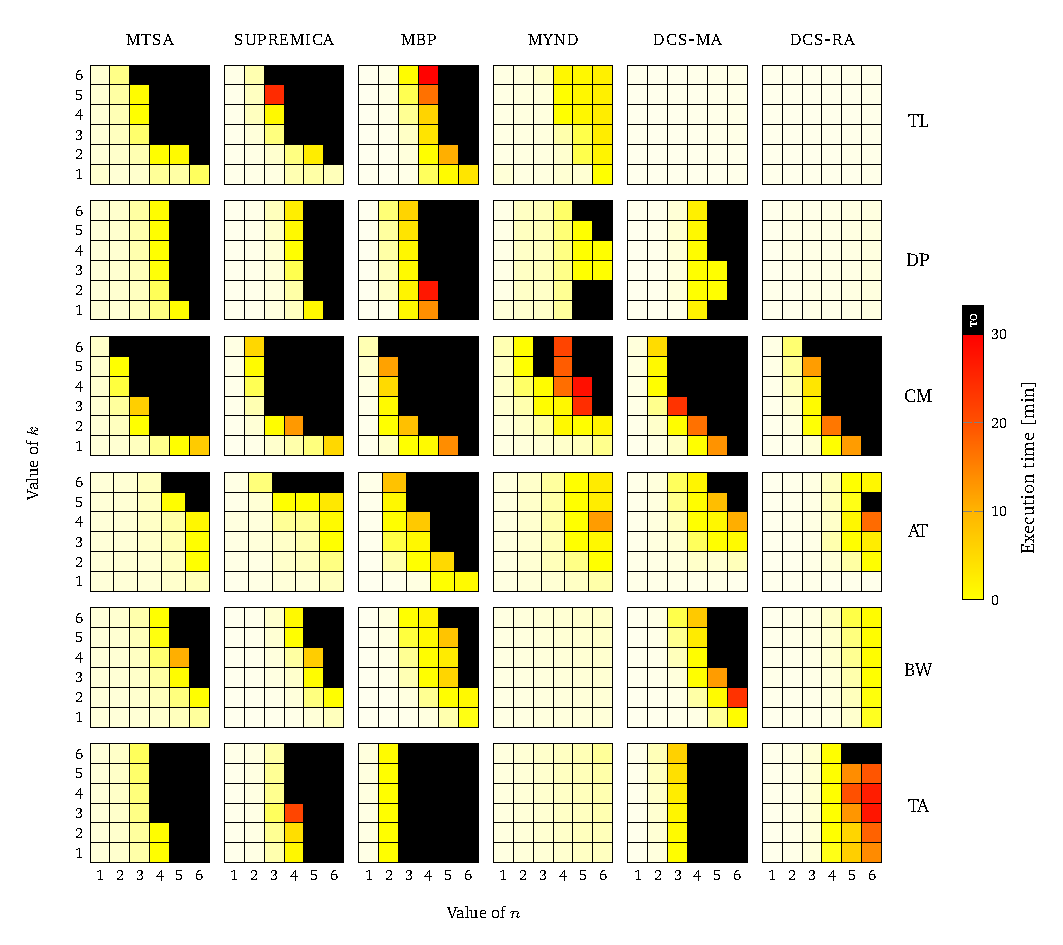
\includegraphics[width=\linewidth]{figures/resultsDani/detailed.pdf}  
			\caption{performance previa}
			\label{fig:detailedPrevio}
		\end{subfigure}
	}
\end{figure}


En la figura{REF} puede verse la comparación y que en la mayoría de los problemas los resultados son similares. Se destacan el problema {NAME} y {NAME} por tener resultados peores y mejores respectivamente luego de la modificación.

De estos resultados concluímos que las modificaciones al algoritmo no afectan de forma significativa su performance.












